\documentclass[aspectratio=169,t,11pt,table]{beamer}
\usepackage{../../slides,../../math}
\definecolor{accent}{HTML}{2B5269}
\definecolor{accent2}{HTML}{9D2235}

\title{Topic 7: Difference-in-Differences and Factor Models}
\subtitle{\it  ECON 5783 — University of Arkansas}
\date{Fall 2024}
\author{Prof. Kyle Butts}

\begin{document}

% -----------------------------------------------------------------------------
\begin{frame}[noframenumbering,plain]
\maketitle

% \bottomleft{\footnotesize $^*$A bit of extra info here. Add an asterich to title or author}
\end{frame}
% -----------------------------------------------------------------------------


\section{Difference-in-Differences}

\begin{frame}{What is difference-in-differences (DiD)}

  \alert{Difference-in-differences} compares a group assigned to treatment versus a group not assigned to treatment
  \begin{itemize}
    \item The estimator compares the treated groups change in outcomes before and after the treatment to the control groups change in outcomes before and after the treatment
  \end{itemize}

  \bigskip
  One of the most widely used quasi-experimental methods in economics and increasingly in industry

\end{frame}

\subsection{Initial Difference-in-difference usage}

\begin{frame}{Ignaz Semmelweis and washing hands}
  Early 1820s, Vienna passed legislation requiring that if a pregnant
  women giving birth went to a public hospital (free care)
  \begin{itemize}
    \item depending on the day of week and time of day, she would be routed
    to either the midwife wing or the physician wing
  \end{itemize}
  
  \bigskip
  Pregnant women died after delivery in the (male) wing at a rate of 13-18\%, but only 3\% in the (female) midwife wing
\end{frame}

\begin{frame}{Ignaz Semmelweis and washing hands}
  Ignaz Semmelweis, after a lot of observation, conjectures that the cause is:
  \begin{itemize}
    \item the teaching faculty would teach anatomy using cadavers and then delivering babies without washing hands
  \end{itemize}

  \bigskip
  Convinced the hospital to have physicians wash their hands in chlorine but not the midwives
  \begin{itemize}
    \item Compared mortality rates in treated Clinic 1 (Physicians and Midwives) vs. untreated Clinic 2 (Midwives only)
  \end{itemize} 
\end{frame}

\imageframe{figures/semmelweis_raw_plots.pdf}

\begin{frame}{Identifying assumptions}
  While this, today, seems like an obvious treatment effect, people at the time did not believe this result
  \begin{itemize}
    \item In fact, Semmelweis was fired about a year and a half later and his life was ruined by critics
  \end{itemize}

  \bigskip
  It is worth asking for this topic, "What do we need to assume to believe this result?"
\end{frame}

\begin{frame}{Identifying assumptions}
  Looking at the previous figure, we see that prior to treatment, mortality rates were way higher in the physicians clinic than midwives.
  Then, right when treatment starts we see a large drop in the mortality rate
  
  \bigskip
  The main issue is that we can not be sure what would happen had the physician clinic not been required to wash their hands
  \begin{itemize}
    \item Do not observe the post-treatment $y(0)$
  \end{itemize}

  \pause
  \bigskip
  We, however, do not see a similar drop in the second clinic, so this rules out many shocks that would impact both clinics
\end{frame}

\begin{frame}{Identifying assumptions}
  What we will come to formalize is the \alert{parallel counterfactual trends} assumption:
  \begin{itemize}
    \item In the absence of treatment, the treated units would be on the same counterfactual trend as we observe in the untreated units
  \end{itemize}

  \bigskip
  You can imagine taking the trend from Clinic 2 and appending that onto the start of the post-period for Clinic 1
  \begin{itemize}
    \item The implied $Y(0)$ if indeed the two clinics would have the same counterfactual trends
  \end{itemize}

  \bigskip
  People typically call it the \emph{parallel trends} assumption
  \begin{itemize}
    \item But I prefer the full phrase because it emphasizes this is about trends for the treated units \emph{had they not been treated}
  \end{itemize}
\end{frame}

\imageframe{figures/semmelweis_implied_y0.pdf}

% TODO: Plumbing historical example
% \begin{frame}{title}
%   
% \end{frame}

\subsection{Classic Example: Card and Krueger (2000, AER)}

\begin{frame}{Card and Krueger (1994, AER)}
  The first ``modern'' economics paper to use difference-in-differences

  \bigskip
  Card and Krueger studied the 1992 minimum wage increase in New Jersey from \$4.25 to \$5.05
  \begin{itemize}
    \item The story goes that they heard about the minimum wage change and \emph{ran to the field} to start collecting data on fast-food employment prior to the minimum wage
    \begin{itemize}
      \item 
    \end{itemize}
  \end{itemize}

  \pause
  \bigskip
  Their strategy was to compare changes to New Jersey fast-food employment to those in Eastern Pennsylavnia
  \begin{itemize}
    \item 331 in New Jersey (treated)
    \item 79 in Eastern Pennsylvania (untreated)
  \end{itemize}
\end{frame}

\begin{frame}{}
  \begin{center}
    
\includegraphics[width= 0.6\textwidth]{figures/minimum_wage_illustration.png}
    
    Source: \href{https://www.nobelprize.org/uploads/2021/10/fig3_ek_en_21_effectIncreasingMinimunWage.pdf}{Nobel Prize summary} 
  \end{center}
\end{frame}

\begin{frame}{Measurements}
  They measured employment before (in March 1992) and after (in December 1992) the minimum wage passed
  \begin{itemize}
    \item This is a relatively small survey, but it was novel because no one really tried to see what the actual impacts of minimum wage changes was
  \end{itemize}
\end{frame}

\imageframe{figures/card_krueger_raw_plots.pdf}

\begin{frame}{Identification}
  So, we see that NJ employment went up slightly and Eastern PA employment went down a bit more
  \begin{itemize}
    \item We infer that NJ would have went down by the same amount as Eastern PA had the minimum wage not passed 
  \end{itemize}

  \bigskip
  That is, we assume that there are ``common shocks'' to both areas and assume that there are no additional shocks that impact \emph{only one} of the two regions
  \begin{itemize}
    \item They are on ``parallel counterfactual trends''
  \end{itemize}
\end{frame}

\imageframe{figures/card_krueger_implied_y0.pdf}

\begin{frame}{Is this believable?}
  From this graph, it's not clear what to think about this assumption of parallel counterfactual trends

  \bigskip
  For this reason, it is (now) typical to compare the treated and control units \emph{prior} to treatment uptake to see if they are on similar trends
  \begin{itemize}
    \item Using many observations before and after treatment are called `event-study' estimates
  \end{itemize}
\end{frame}

\begin{frame}{}
  \begin{center}
    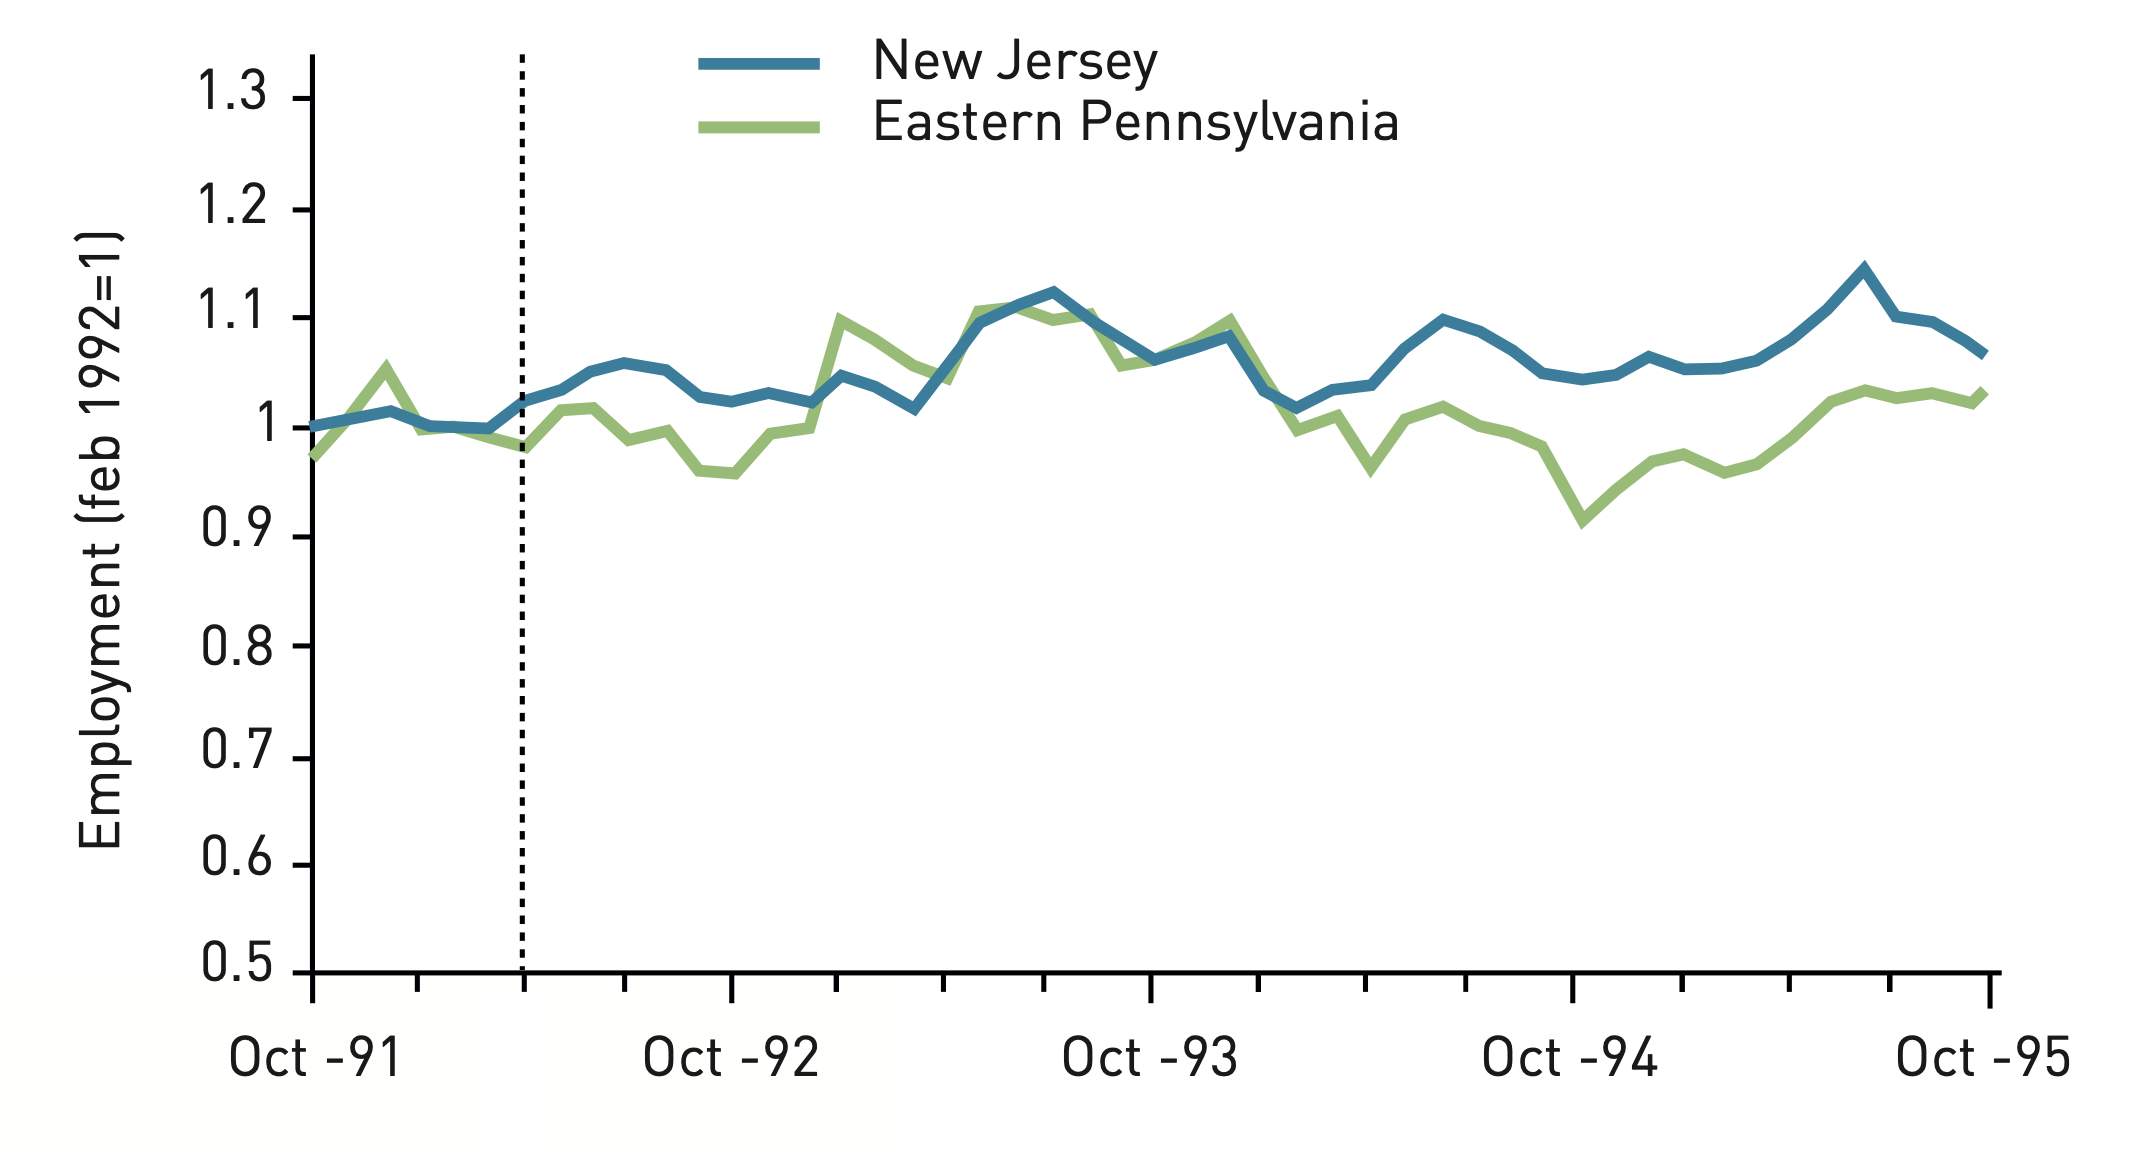
\includegraphics[width= 0.9\textwidth]{figures/card_krueger_event_study.png}
    
    Source: \href{https://www.nobelprize.org/uploads/2021/10/fig3_ek_en_21_effectIncreasingMinimunWage.pdf}{Nobel Prize summary} 
  \end{center}
\end{frame}

\begin{frame}{Pre-trends}
  The previous figure shows that for a few months prior to the minimum wage change, the employment trends of Eastern PA and New Jersey followed closely to one another
  \begin{itemize}
    \item This supports the idea that in the absence of treatment the NJ and Eastern PA trends would be similar in the post-period
  \end{itemize}

  \pause
  \bigskip
  To be clear, parallel counterfactual trends involves the \emph{post-treatment $y_{it}$}
  \begin{itemize}
    \item Having similar trends prior to treatment helps support this assumption, but does not \emph{prove it}
  \end{itemize}
\end{frame}

\begin{frame}{Ashenfelter's dip}
  Orley Ashenfelter's 1978 paper entitled ``Estimating the Effect of Training Programs on Earnings'' is a great example to illustrate the different between common trends before treatment and the \emph{parallel counterfactual trends} assumption

  \pause
  \bigskip
  He looks at individuals that sign-up for a work training program on their future earnings
  \begin{itemize}
    \item For many years prior to treatment, the workers that do and do not enter the training have common earnings trends
    
    \item Just prior to treatment, the workers that do enter the program face a sudden \emph{dip} in earnings
    
    \item Then, after the program, the workers' earnings go back up towards the original level
  \end{itemize}
\end{frame}

\begin{frame}{Ashenfelter's dip}
  What was happening was that workers just prior to treatment lost their job (hence trying to learn new labor force skills)

  \pause
  \bigskip
  In the absence of the training, we would expect those workers to have a raise in earnings anyways because they would likely be hired somewhere
  \begin{itemize}
    \item The treated workers and the untreated workers have different earning dynamics
  \end{itemize}

  \bigskip
  So even though they have similar trends prior to treatment, the parallel counterfactual trends assumption does not hold in this setting
\end{frame}

\imageframe{figures/ashenfelters_dip.pdf}
\imageframe{figures/ashenfelters_dip_implied_y0.pdf}

\begin{frame}{DID Key Ideas}
  \alert{Difference-in-differences} compares a group assigned to treatment versus a group not assigned to treatment
  \begin{itemize}
    \item The estimator compares the treated groups change in outcomes before and after the treatment to the control groups change in outcomes before and after the treatment
  \end{itemize}

  \bigskip
  The key assumption we make is the \alert{parallel counterfactual trends} assumption
  \begin{itemize}
    \item The change in outcomes over time for control units are an appropriate stand-in for the treated unit's change in outcomes \emph{if they did not receive treatment}
  \end{itemize}
\end{frame}



\subsection{Econometric formulation to DID}

\begin{frame}{2 $\times$ 2 Difference-in-Differences}
  The Card and Krueger minimum wage paper is an example of the canonical $2 \times 2$ DID, so we will begin there
  
  \bigskip
  We observe units $i \in \{ 1, \dots, N \}$ for two periods (before and after), $t = 0$ and $t = 1$
  \begin{itemize}
    \item Let $D_i$ be an indicator for which units receive treatment
    \item Let $\text{Post}_t = \one{t = 1}$ be an indicator for being in the post-period
  \end{itemize}


  \pause
  \bigskip
  Then, we have potential outcomes for each unit in the post-period:
  \begin{itemize}
    \item $y_{i0}(D_i)$ and $y_{i1}(D_i)$
    \begin{itemize}
      \item We typically assume that treatment does not impact $y_{i0}$, i.e. $y_{i0} = y_{i0}(1) = y_{i0}(0)$. This is called the ``no anticipation'' assumption
    \end{itemize}
  \end{itemize}  
\end{frame}

\begin{frame}{Treatment effect of interest}
  The treatment effect of interest is the average effect of treatment in period $1$ for the treated units:
  $$
    \text{ATT}_1 = \expec{y_{i1}(1) - y_{i1}(0)}{D_i = 1}
  $$
  
  The counterfactual compares the period $1$ outcome under treatment to the period $1$ outcome in the absence of treatment
  \begin{itemize}
    \item {\color{red} This is \emph{\textbf{not}} the post-$y$ minus pre-$y$!}
  \end{itemize}
\end{frame}

\begin{frame}{Parallel Counterfactual Trends assumption}
  Our \alert{Parallel Counterfactual Trends} imposes restrictions on the change in untreated potential outcomes:
  $$
    \expec{y_{i1}(0) - y_{i0}(0)}{D_i = 1} = \expec{y_{i1}(0) - y_{i0}(0)}{D_i = 0} 
  $$

  \bigskip
  This says, in the absence of treatment, the change in $y$ is on average the same for the treated and the control group
\end{frame}

\begin{frame}{Observed difference in $y$}
  For the treated unit, we can do an econometrician's favorite math trick (add and subtract something) to analyze the observed change in $y$ for the treated units:
  \begin{align*}
    \expec{y_{i1} - y_{i0}}{D_i = 1} 
    &= \expec{y_{i1}(1) - y_{i0}(0)}{D_i = 1} \\
    \pause
    &= \expec{y_{i1}(1) \tcbhighmath[colback = bgGreen]{- y_{i1}(0) + y_{i1}(0)} - y_{i0}(0)}{D_i = 1} \\
    \pause
    &= \expec{y_{i1}(1) - y_{i1}(0)}{D_i = 1} + \expec{y_{i1}(0) - y_{i0}(0)}{D_i = 1} \\
    \pause
    &= \text{ATT}_1 + \expec{y_{i1}(0) - y_{i0}(0)}{D_i = 1}
  \end{align*}

  \medskip 
  $\implies$ The change in outcome for the treated units is the effect of treatment plus the treated groups' counterfactual trend
\end{frame}

\begin{frame}{Observed difference in $y$}
  \vspace*{-\bigskipamount}
  $$
    \expec{y_{i1} - y_{i0}}{D_i = 1} = \text{ATT}_1 + \expec{y_{i1}(0) - y_{i0}(0)}{D_i = 1}
  $$

  \bigskip\bigskip
  For control units, the math is simpler 
  $$
    \expec{y_{i1} - y_{i0}}{D_i = 0} = \expec{y_{i1}(0) - y_{i0}(0)}{D_i = 0}
  $$

  \medskip
  $\implies$ The change in outcome for the controlunits is the effect of treatment plus the control groups' counterfactual trend 
\end{frame}

\begin{frame}{Difference-in-differences}
  Now, the difference-in-differences estimand is formed by subtracting the two change in outcomes:
  \begin{align*}
    \tau_{\texttt{DID}} &= \expec{y_{i1} - y_{i0}}{D_i = 1} - \expec{y_{i1} - y_{i0}}{D_i = 0}  \\ 
    \pause
    &= \text{ATT}_1 + \expec{y_{i1}(0) - y_{i0}(0)}{D_i = 1} - \expec{y_{i1}(0) - y_{i0}(0)}{D_i = 0}
  \end{align*}

  \bigskip
  The difference-in-differences estimand compares treated unit's change in $y$ to control unit's change in $y$
  \begin{itemize}
    \item This estimates the effect of treatment plus the difference in trends between the two groups
  \end{itemize}
\end{frame}

\begin{frame}{Difference-in-differences}
  \vspace*{-\bigskipamount}
  \begin{align*}
    \tau_{\texttt{DID}} &= \expec{y_{i1} - y_{i0}}{D_i = 1} - \expec{y_{i1} - y_{i0}}{D_i = 0}  \\ 
    &= \text{ATT}_1 + \expec{y_{i1}(0) - y_{i0}(0)}{D_i = 1} - \expec{y_{i1}(0) - y_{i0}(0)}{D_i = 0}
  \end{align*}

  \medskip
  For example, if the treated group had a larger counterfactual growth in $y$ (like in Ashenfelter's dip example), then the treatment effect will be biased upwards
\end{frame}

\begin{frame}{Difference-in-differences}
  However, assuming parallel counterfactual trends implies that these two counterfactual trend terms are the same and therefore cancel out
  \begin{align*}
    \tau_{\texttt{DID}} &= \expec{y_{i1} - y_{i0}}{D_i = 1} - \expec{y_{i1} - y_{i0}}{D_i = 0}  \\ 
    &= \text{ATT}_1 + \expec{y_{i1}(0) - y_{i0}(0)}{D_i = 1} - \expec{y_{i1}(0) - y_{i0}(0)}{D_i = 0} \\ 
    \pause
    &= \text{ATT}_1 + \expec{y_{i1}(0) - y_{i0}(0)}{D_i = 1} - \expec{y_{i1}(0) - y_{i0}(0)}{D_i = 1} \\
    &= \texttt{ATT}_1
  \end{align*}
\end{frame}

\begin{frame}{Difference-in-differences as an imputation estimator}
  Remember in the selection on observables topic, we used a regression imputation estimator to explicitly estimate the treated units' $y_i(0)$.

  \bigskip
  It turns out, we can write the difference-in-differences estimator as an imputation estimator
\end{frame}

\begin{frame}{Difference-in-differences as an imputation estimator}
  Our imputation for $y_{i1}(0)$ is given as:
  $$
    \hat{y}_{i1}(0) = y_{i0} + \expec{y_{i1}(0) - y_{i0}(0)}{D_i = 0}
  $$
  In words, take the unit's period $t = 0$ outcome and add to it the average change in $y$ for the comparison group.
  \begin{itemize}
    \item This is what I was drawing in the figures at the start of the slides
  \end{itemize}
\end{frame}

\begin{frame}{$2 \times 2$ DID Estimation}
  Our estimation strategy replaces these terms with their sample averages:
  $$
    \hat{\tau}_{\texttt{DID}} = \expechat{y_{i1} - y_{i0}}{D_i = 1} - \expechat{y_{i1} - y_{i0}}{D_i = 0}
  $$

  \bigskip
  We could do this as four averages
  $$
    \left(\expechat{y_{i1}}{D_i = 1} - \expechat{y_{i0}}{D_i = 1}\right) - \left(\expechat{y_{i1}}{D_i = 0} - \expechat{y_{i0}}{D_i = 0} \right)
  $$

  \pause
  \bigskip
  Or just do a difference-in-means using $y_{i1} - y_{i0}$ as the outcome variable
  \begin{itemize}
    \item \bgYellow{Be careful to only have one row per unit when running this regression}
  \end{itemize}
\end{frame}

\begin{frame}{A note on the name `Difference-in-Differences'}
  The correct name is Difference in Difference\emph{s}
  \begin{itemize}
    \item You are taking the difference between \emph{two} avrages of first-differences
  \end{itemize}

  \bigskip
  Personal pet-peeve, but this is the one and only name for this estimator
\end{frame}

\begin{frame}{$2 \times 2$ in regression form}
  Just like difference-in-means, it turns out you can use OLS regression to estimate $\hat{\tau}_{\text{DID}}$

  $$
    y_{it} = \alpha + \gamma D_i + \lambda \text{Post}_t + \tau d_{it} + u_{it}
  $$
  \begin{itemize}
    \item $d_{it} = D_i \text{Post}_t$ is an indicator for when a unit is actively under treatment
  \end{itemize}

\end{frame}

\begin{frame}{$2 \times 2$ in regression form}
  \vspace*{-\bigskipamount}
  $$
    y_{it} = \alpha + \gamma D_i + \lambda \text{Post}_t + \tau d_{it} + u_{it}
  $$
  
  \bigskip
  Since these are just a bunch of indicator variables, we can derive what they estimate:
  \begin{align*}
    \tag{1}
    \expec{Y_{it}}{D_i = 0, \text{Post}_t = 0} 
    &= \expec{Y_{i0}}{D_i = 0} 
    &= \alpha \\ 
    \tag{2}
    \expec{Y_{it}}{D_i = 0, \text{Post}_t = 1} 
    &= \expec{Y_{i1}}{D_i = 0} 
    &= \alpha + \lambda \\ 
    \tag{3}
    \expec{Y_{it}}{D_i = 1, \text{Post}_t = 0} 
    &= \expec{Y_{i0}}{D_i = 1} 
    &= \alpha + \gamma \\ 
    \tag{4}
    \expec{Y_{it}}{D_i = 1, \text{Post}_t = 1} 
    &= \expec{Y_{i1}}{D_i = 1} 
    &= \alpha + \gamma + \lambda + \tau 
  \end{align*}

  Solving these equations for $\tau$ give the DID estimate: $\tau = \left[ (4) - (3) \right] - \left[ (2) - (1) \right]$
\end{frame}


\begin{frame}{$2 \times 2$ in regression form}
  \vspace*{-\bigskipamount}
  $$
    y_{it} = \alpha + \gamma D_i + \lambda \text{Post}_t + \tau d_{it} + u_{it}
  $$
  
  \bigskip
  First, we have $\hat{\alpha} = \expechat{y_{i0}}{D_i = 0}$ and $\hat{\gamma} = \expechat{y_{i0}}{D_i = 1}$

  \bigskip
  Second, we have $\hat{\lambda} = \expechat{y_{i1} - y_{i0}}{D_i = 0}$ 

  \bigskip
  Last, we have 
  $$
    \hat{\tau}_{\text{OLS}} = \expechat{y_{i1} - y_{i0}}{D_i = 1} - \expechat{y_{i1} - y_{i0}}{D_i = 0}
  $$
\end{frame}

\begin{frame}{$2 \times 2$ in regression form}
  You can also use unit and time fixed-effects to estimate this
  $$
    y_{it} = \mu_i + \lambda_t + \tau d_{it} + u_{it}
  $$
  
  \bigskip
  It is also true that, $\hat{\tau}_{\text{OLS}} = \hat{\tau}_{\text{DID}}$!
  \begin{itemize}
    \item Note that one of the time fixed-effects will need to be omitted for collinearity
  \end{itemize}

  \bigskip
  This form is usually more common, so we will focus on that
  \begin{itemize}
    \item "Absorb the time-fixed effects of individuals and common time-shocks"
  \end{itemize}
\end{frame}

\begin{frame}{\bgYellow{Users Beware !!}}
  The equivalence between OLS and $2 \times 2$ DID only holds in this case. 
  Using OLS in other cases will turn out to bite us in the butt later on
  \begin{itemize}
    \item People have been using OLS for DID for a long time and it turns out to create problems when treatment starts at different points in time for different units
  \end{itemize}
\end{frame}

\subsection{Event-study}

\begin{frame}{Multiple pre- and post- periods}
  Now, consider an extension of the $2 \times 2$ DID where we observe $N$ units over $t = 1, \dots, T_0, T_0 + 1, \dots, T$ time periods
  
  \bigskip
  Treatment turns on for some individuals at period $T_0 + 1$. Here, we still have $D_i$ be the treatment indicator
\end{frame}

\begin{frame}{Dynamic treatment effects}
  However, we now have many post-periods, so we will look at $\text{ATT}^\ell$ coefficients:
  $$
    \text{ATT}^\ell = \expec{ y_{it}(1) - y_{it}(0) }{D_i = 1}
  $$  

  \begin{itemize}
    \item The impact of being treated in period $t > T_0$
    
    \item No anticipation implies $\text{ATT}^\ell = 0$ for $l \leq T_0$
  \end{itemize}

  \pause
  \bigskip
  These are called \alert{dynamic treatment effects}
  \begin{itemize}
    \item E.g. policies might take a while to be in full-effect ($\text{ATT}^\ell$ growing)
    
    \item Or, the policy has a large initial shock that fades away as people adapt
  \end{itemize}
\end{frame}

\begin{frame}{Dynamic Treatment Effects}
  These can be identified using a similar $2 \times 2$ strategy:
  $$
    \text{ATT}^\ell = \expec{y_{it} - y_{iT_0}}{D_i = 1} - \expec{y_{it} - y_{iT_0}}{D_i = 0}
  $$

  \bigskip
  Comparing ``long-differences'' from period $T_0$ to period $t$. This requires parallel trends holds for all post-periods:
  $$
    \expec{y_{it}(0) - y_{iT_0}(0)}{D_i = 1} = \expec{y_{it}(0) - y_{iT_0}(0)}{D_i = 0}
  $$
\end{frame}

\begin{frame}{Estimating dyanmic effects using OLS}
  Similarly, we can estimate these using OLS:
  $$
    y_{it} = \mu_i + \lambda_t + \sum_{\ell = T_0 + 1}^T d_{it}^\ell \tau^\ell + v_{it},
  $$
  
  where $d_{it}^\ell = \one{D_i = 1} * \one{t = \ell}$ are called the \alert{event-study indicators}

  \bigskip
  Just like the $2 \times 2$, the OLS estimates are the sample analogue 
  $$
    \hat{\tau}^{\ell} = \expechat{y_{it} - y_{iT_0}}{D_i = 1} - \expechat{y_{it} - y_{iT_0}}{D_i = 0}
  $$ 
\end{frame}

\begin{frame}{Pre-trends estimates}
  If you recall, one thing that made us confident in our time-series plots was that the treated and control units had similar trends prior to treatment (bolstering confidence in our parallel trends assumption)

  \pause
  \bigskip
  It is common, to include similar $d_{it}^\ell$ event-study indicators for $t < T_0$
  $$
    y_{it} = \mu_i + \lambda_t + \sum_{\ell = 1, \dots, T_0 - 1, T_0 + 1, \dots, T} d_{it}^\ell \tau^\ell + v_{it},
  $$
  
  The pre-treatment $\ell$ estimate `placebo estimates' and if parallel trends holds in the pre-periods, they should be zero.
\end{frame}

\begin{frame}{``Event-time''}
  An equivalent way of writing this is to instead use event-time: $t - (T_0 + 1)$
  \begin{itemize}
    \item event-time $= 0$ is the first period of treatment
    \item event-time $= 1$ is the second period of treatment
    \item event-time $= -1$ is the period before treatment
  \end{itemize}

  \bigskip
  Then, you estimate 
  $$
    y_{it} = \mu_i + \lambda_t + \sum_{\ell = -T_0, \dots, -2, 0, \dots, T - T_0} d_{it}^\ell \tau^\ell + v_{it},
  $$
  
  \begin{itemize}
    \item In this case, the points are the same; just relabeling
  \end{itemize}
\end{frame}

\begin{frame}{Event-study plots}
  It is common to plot the coefficients $\hat{\tau}^\ell$ to show two things:
  \begin{enumerate}
    \item The pre-treatment estimates should be near zero and not show any trends
    
    \item The post-treatment effect dynamics
  \end{enumerate}
\end{frame}

\imageframe{figures/event_study_ex_1_raw.pdf}
\imageframe{figures/event_study_ex_1_estimates.pdf}
\imageframe{figures/event_study_ex_2_raw.pdf}
\imageframe{figures/event_study_ex_2_estimates.pdf}
\imageframe{figures/event_study_ex_3_raw.pdf}
\imageframe{figures/event_study_ex_3_estimates.pdf}



\section{Conditional Parallel Trends}

\begin{frame}{Conditional Parallel trends}
  Just like in the first two topics of the course, economists often times find the parallel trends assumption to be too strong and want to use covariates to relax this assumption
  \begin{itemize}
    \item Similar to completely randomly assigned compared to assigned randomly conditional on observables
  \end{itemize}

  \pause
  \bigskip
  Say we have $X_i$ be a unit's gender. We might think men and women have different wage trends in the sample
  \begin{itemize}
    \item I.e. we think looking among people of the same gender, trends are parallel
  \end{itemize}
\end{frame}

\begin{frame}{Conditional Parallel Trends}
  Just like selection on observables, there is an obvious estimation strategy
  \begin{itemize}
    \item Look within workers with the same gender and estimate a male DID and a female DID
  \end{itemize}

  \bigskip
  For the overall ATT, we can take a weighted average of gender-specific DID estimates
\end{frame}

\begin{frame}{Conditional Parallel Trends}
  Let $\bm{X}_i$ be a set of time-invariant characteristics of a unit $i$
  \begin{itemize}
    \item E.g. gender, years of education, etc.
  \end{itemize}

  \bigskip
  Our \alert{Conditional Parallel Trends} Assumption says
  $$
    \expec{y_{i1}(1) - y_{i0}(0)}{D_i = 1, \bm{X}_i = \bm{x}} = 
    \expec{y_{i1}(1) - y_{i0}(0)}{D_i = 0, \bm{X}_i = \bm{x}}
  $$
  for all values of $\bm{x}$ 
\end{frame}

\begin{frame}{Conditional Parallel Trends does not imply Parallel Trends}
  Say we have $X_i$ be a unit's gender and conditional parallel trends holds. The unconditional trends for the treated and untreated groups are:
  \begin{align*}
    &\expec{y_{i1}(1) - y_{i0}(0)}{D_i = d} =\\
    &\quad\quad \prob{X_i = F}{D_i = d} \expec{y_{i1}(1) - y_{i0}(0)}{D_i = d, X_i = F} \\
    &\quad\quad+ \prob{X_i = M}{D_i = d} \expec{y_{i1}(1) - y_{i0}(0)}{D_i = d, X_i = M} 
  \end{align*}

  \pause
  \bigskip
  If the gender composition of the treated group differs from the untreated group, PTs does not hold (even though conditional PTs does)
\end{frame}

\begin{frame}{Estimation Strategies with Conditional Parallel Trends}
  One way of rewriting the conditional parallel trends assumption is as follows:
  $$
    \expec{\Delta y_i}{D_i = d, \bm{X}_i = \bm{x}} = \expec{\Delta y_i}{\bm{X}_i = \bm{x}}
  $$

  That is, treatment is mean-independent of the \emph{change in $y_i$} conditional on $\bm{X}_i$
  
  \pause
  \bigskip
  $\implies$ We can treat this like a selection-on-observables problem where $\Delta y_i = y_{i1} - y_{i0}$ is our outcome variable
  \begin{itemize}
    \item This unlocks all of our selection-on-observables strategies
  \end{itemize}
\end{frame}

\begin{frame}{Example 1: Matching}
  \vspace*{-\bigskipamount}
  $$
    \expec{\Delta y_i}{D_i = d, \bm{X}_i = \bm{x}} = \expec{\Delta y_i}{\bm{X}_i = \bm{x}}
  $$

  \bigskip
  For instance, we could perform a nearest-neighbor matching exercise where we match up treated and control units with similar $\bm{X}_i$ and perform a difference-in-means of $\Delta y_i$ with the matched control group
\end{frame}

\begin{frame}{Example 1: Matching}
  For event-study type setups, we can do a version of this where
  we use $y_{it} - y_{iT_0}$ as the outcome variable
  \begin{itemize}
    \item For each $t \in 1, \dots, T_0 - 1, T_0 + 1, \dots, T$, we can compute an estimate using the matched-control group
  \end{itemize}

  \bigskip
  Collect the $\hat{\tau}^\ell$ and we can make our event-study plot
\end{frame}

\begin{frame}{Regression Adjustment}
  It is worth spending a moment thinking about the regression adjustment estimator. 
  
  Using just the control units, we estimate this model:
  $$
    y_{i1}(0) - y_{i0}(0) = \alpha + \bm{X}_i \beta + u_i
  $$

  \pause
  \bigskip
  $\hat{\beta}$ will estimate how the change in $y_i(0)$ varies by $\bm{X}_i$
  \begin{itemize}
    \item For e.g. if $\bm{X}_i$ was an inidicator for being a female
    \begin{itemize}
      \item $\hat{\alpha}$ would estimate the average male trend in $y(0)$
      
      \item $\hat{\beta}$ would estimate the difference in average female trend in $y(0)$ relative to the male trend 
    \end{itemize}
  \end{itemize}
\end{frame}

\begin{frame}{Regression Adjustment}
  \vspace*{-\bigskipamount}
  $$
    y_{i1}(0) - y_{i0}(0) = \alpha + \bm{X}_i \beta + u_i
  $$
  
  What regression adjustment is doing, in effect, is estimating how trends across units based on their $\bm{X}_i$ and adjusting for it
\end{frame}

\begin{frame}{Regression Adjustment}
  \vspace*{-\bigskipamount}
  $$
    y_{i1}(0) - y_{i0}(0) = \alpha + \bm{X}_i \beta + u_i
  $$
  
  \bigskip
  Once we have $\hat{\alpha}$ and $\hat{\beta}$ estimated using our $D_i = 0$ units, we can form our DID estimate as 
  $$
    \hat{\tau}_{\text{RA}} = \frac{1}{N_1} \sum_{i \ : \ D_i = 1} \left( \Delta y_i \right) - \underbrace{ (\hat{\alpha} + \bm{X}_i \hat{\beta}) }_{\widehat{\Delta y(0)}}
  $$
\end{frame}





% TODO: Unit fixed-effects ``cancel out''


% \begin{frame}{Simple Difference-in-differences and Four Means}
%   % \begin{table}[h!]
%   %   \centering
%   %   \begin{tabular}{|c|c|c|}
%   %     \hhline{~--}
%   %     \multicolumn{1}{c|}{} & 
%   %     \multicolumn{1}{c|}{\cellcolor{bgOrange}$t = 0$} & 
%   %     \multicolumn{1}{c|}{\cellcolor{bgOrange}$t = 1$} \\
%   %     \hline
%   %     
%   %     \cellcolor{bgOrange}$D_i = 0$ & $\gamma_0 + \alpha_i$ & $\gamma_1 + \alpha_i$ \\
%   %     \hline
%   %     
%   %     \cellcolor{bgOrange}$D_i = 1$ & $\gamma_0 + \alpha_i$ & $\gamma_1 + \alpha_i + \tau_i$ \\
%   %     \hline
%   %   \end{tabular}
%   % \end{table}
% 
%   \bigskip
%   Taking first differences and ignoring error term:
%   \begin{itemize}
%     \item For $D_i = 0$, $y_{i1} - y_{i0} = \gamma_1 - \gamma_0 + u_{i1} - u_{i0}$
%     
%     \item For $D_i = 1$, $y_{i1} - y_{i0} = \gamma_1 - \gamma_0 + \tau_i + u_{i1} - u_{i0}$
%   \end{itemize}
% 
%   \bigskip
%   The key assumption is that 
% \end{frame}







% \section{Staggered Treatment Timing}







\end{document}
    
